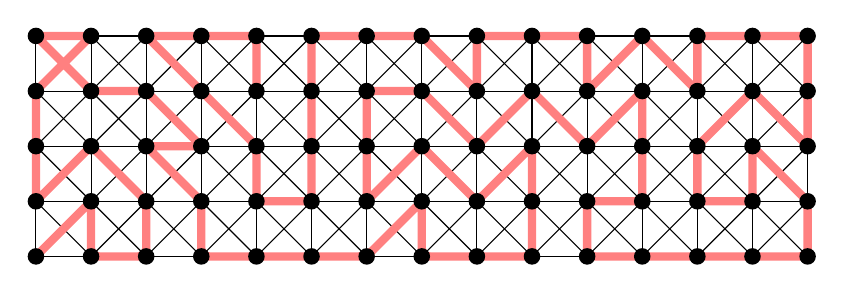
\begin{tikzpicture}[scale=0.7]
  \draw (0,0) grid (14,4);
  \foreach \x in {0,1,...,13} {
    \foreach \y in {0,1,2,3} {
      \draw (\x, \y)--(\x + 1, \y + 1);
      \draw (\x + 1, \y)--(\x, \y + 1);
    }
  }
  \draw[red!50, line width=3,rounded corners=1mm] (0,0)--(1,1)--(1,0)--(2,0)--(2,1)--(1,2)--(0,1)--(0,2)--(0,3)--(1,4)--(0,4)--(1,3)--(2,3)--(3,2)--(2,2)--(3,1)--(3,0)--(6,0)--(7,1)--(7,0)--(9,0)--(9,2)--(8,1)--(7,2)--(6,1)--(6,3)--(7,3)--(8,2)--(9,3)--(10,2)--(11,3)--(11,1)--(10,1)--(10,0)--(11,0)--(14,0)--(14,1)--(13,2)--(13,1)--(12,1)--(12,2)--(13,3)--(14,2)--(14,4)--(12,4)--(12,3)--(11,4)--(10,3)--(10,4)--(8,4)--(8,3)--(7,4)--(5,4)--(5,1)--(4,1)--(4,2)--(2,4)--(4,4)--(4,3);
  \foreach \x in {0,1,...,14} {
    \foreach \y in {0,1,...,4} {
      \fill (\x, \y) circle (0.15);
    }
  }
\end{tikzpicture}